

\documentclass[a4paper]{article}
\usepackage{Sweave}

\usepackage{amsmath}
\bibliographystyle{plain}



\usepackage{float}
\newcommand{\uvec}{{\bf u}}
\newcommand{\mvec}{{\bf m}}
\newcommand{\nvec}{{\bf n}}
\newcommand{\vvec}{{\bf v}}
\newcommand{\half}{\textstyle{\frac{1}{2}}}
\newcommand{\jhalf}{\half}

\begin{document}
\Sconcordance{concordance:GeometricPhyllotaxisTestVignette.tex:GeometricPhyllotaxisTestVignette.Rnw:%
1 25 1 1 9 5 0 4 1 4 0 1 3 8 1 1 14 1 2 9 1 1 15 1 2 18 1 1 41 1 1 1 2 %
7 0 1 2 2 1 1 4 21 0 1 1 21 0 1 2 1 9 17 0 1 2 9 1 1 2 6 0 2 1 6 0 1 2 %
2 1 1 2 7 0 1 2 1 1 1 2 7 0 1 2 2 1 1 2 1 0 1 1 6 0 1 2 1 19 1 4 18 0 1 %
1 18 0 1 2 3 1 1 2 7 0 1 2 13 1 1 2 11 0 1 2 1 1 1 6 11 0 1 3 6 1 1 2 7 %
0 1 2 1 1 1 3 18 0 1 1 18 0 1 2 1 1 1 10 2 1 2 2 10 1 1 39 5 1 2 2 13 1 %
1 17 1 4 3 1 1 2 32 1 1 2 1 0 1 1 5 0 1 4 2 1 1 2 8 0 1 2 4 1 1 5 12 1 %
1 2 11 0 1 2 5 1 1 2 3 1 1 4 1 5 1 1 1 27 97 1 1 2 29 0 2 3 1 0 2 1 24 %
0 1 1 28 0 1 22 6 1 1 2 1 0 1 1 25 0 1 3 1 0 2 1 3 0 2 2 1 0 1 1 25 0 1 %
2 3 1 1 23 1 2 4 1 1 2 1 0 2 1 55 0 1 5 3 1 1 3 1 0 2 1 4 0 1 2 9 1 1 2 %
5 0 1 2 3 1 1 2 5 0 1 2 20 1}


\title{Theory and code for geometrical phyllotaxis}
\author{Jonathan Swinton}
\maketitle

%\section{Housekeeping}
\begin{Schunk}
\begin{Sinput}
> if(FALSE) {
+   install.packages("xtable")
+   install.packages("showtext")
+   install.packages("showtextdb")
+ }
> library(GeometricalPhyllotaxis)
> library(grid)
> library(xtable)
> library(showtext); showtext.auto() # for greek symbols in plots
> 
\end{Sinput}
\end{Schunk}


\section{Periodic lattices}
We have vertical infinite cylinders of radius $\rho$ and circumference $R=2\pi\rho$.
coordinate $x \in [0,2\pi\rho]$  and vertical coordinate $z$ as in Figure~\ref{fig:cylcoord}.
We can take the divergence $d=x/2\pi\rho$, $d\in [0,1]$ as an alternative horizontal coordinate.

\begin{center}
\begin{figure}[H]
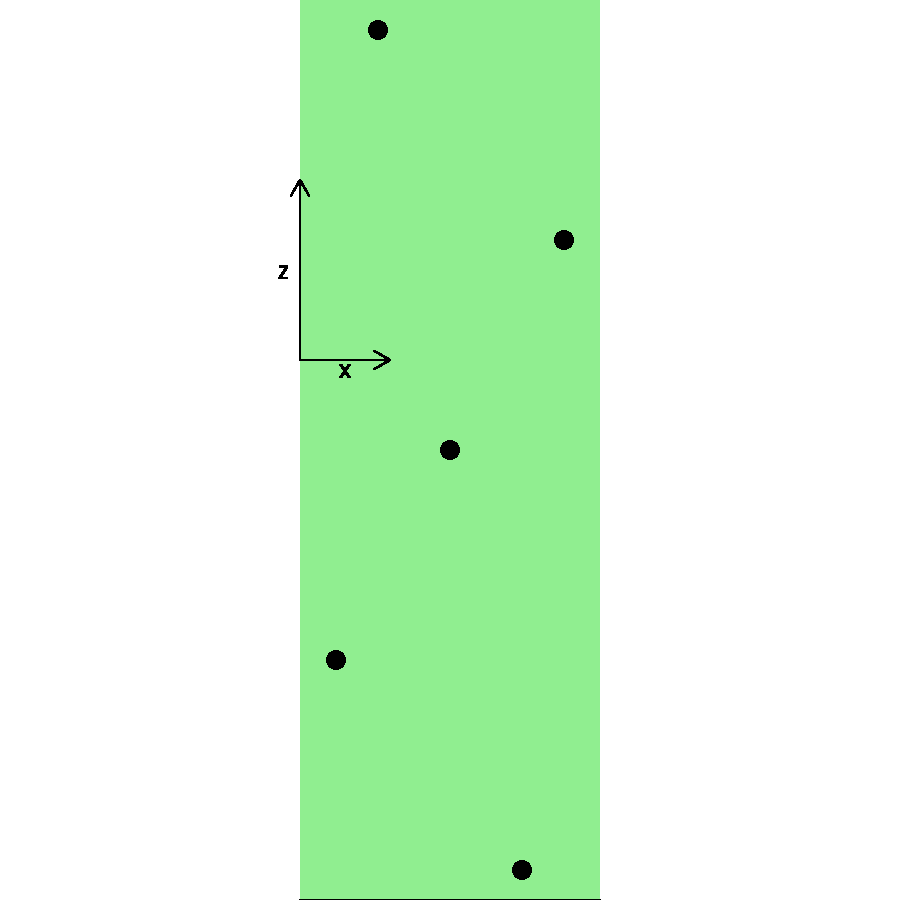
\includegraphics{figdir/fig-plotPGtest}
\caption{A cylinder unwound into the plane}
\label{fig:cylcoord}
\end{figure}
\end{center}

A choice of divergence $d$ and rise $h$ defines a lattice on the cylinder.
The code may not work properly for Jugacy $J>1$. TEST.

\begin{center}
\begin{figure}[H]
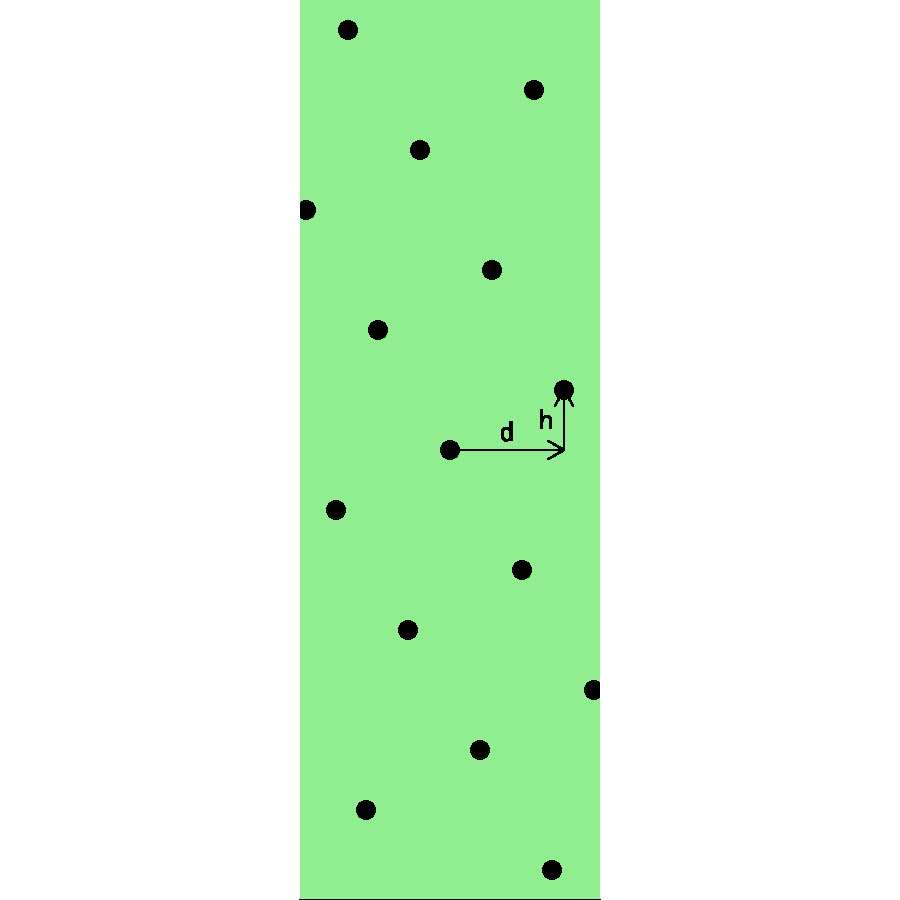
\includegraphics{figdir/fig-scaledpgtest}
\caption{The lattice defined by its genetic parameters}
\label{fig:latticegenetic}
\end{figure}
\end{center}





\clearpage
\section{Winding numbers}
Given a pair of coprime positive integers $m,n$  a {congruence pair} for $m,n$ is $u,v$ where
\begin{equation}
v m - u n = 1
\label{eq:wnp}
\end{equation}
For $1<m<n$ the \emph{winding number pair} for $m,n$ is the unique congruence pair of integers $u,v$ satisfying $0<u<m,0<v<n$;
For $\Delta=\pm1$, the generalised winding number is the unique pair of integers $u(m,n,\Delta),v(m,n,\Delta)$ satisfying $v m - u n = \Delta$.


Winding numbers can be calculated using the \texttt{windingNumbers} function and are tabulated in Table~\ref{tab:wnp} and Table~\ref{tab:wnm}. As implemented it extends the range of $m$ and $n$.
\begin{Schunk}
\begin{Sinput}
> windingNumbers(m=34,n=55,Delta=1)
\end{Sinput}
\begin{Soutput}
[1] 21 34
\end{Soutput}
\end{Schunk}



% latex table generated in R 3.4.0 by xtable 1.8-2 package
% Tue Jun 20 22:38:07 2017
\begin{table}[ht]
\centering
\begin{tabular}{rllllllllll}
  \hline
 & n=1 & 2 & 3 & 4 & 5 & 10 & 11 & 20 & 34 & 55 \\ 
  \hline
m=1 & (1/2,1/2) & (0,1) & (0,1) & (0,1) & (0,1) & (0,1) & (0,1) & (0,1) & (0,1) & (0,1) \\ 
  2 & (1,1) &  & (1,2) &  & (1,3) &  & (1,6) &  &  & (1,28) \\ 
  3 & (2,1) & (1,1) &  & (2,3) & (1,2) & (2,7) & (1,4) & (1,7) & (2,23) & (2,37) \\ 
  4 & (3,1) &  & (1,1) &  & (3,4) &  & (1,3) &  &  & (1,14) \\ 
  5 & (4,1) & (2,1) & (3,2) & (1,1) &  &  & (4,9) &  & (1,7) &  \\ 
  7 & (6,1) & (3,1) & (2,1) & (5,3) & (4,3) & (2,3) & (5,8) & (1,3) & (1,5) & (1,8) \\ 
  10 & (9,1) &  & (3,1) &  &  &  & (9,10) &  &  &  \\ 
  19 & (18,1) & (9,1) & (6,1) & (14,3) & (15,4) & (17,9) & (12,7) & (18,19) & (5,9) & (10,29) \\ 
  32 & (31,1) &  & (21,2) &  & (19,3) &  & (29,10) &  &  & (25,43) \\ 
  34 & (33,1) &  & (11,1) &  & (27,4) &  & (3,1) &  &  & (21,34) \\ 
   \hline
\end{tabular}
\caption{Winding numbers for $\Delta=1$} 
\label{tab:wnp}
\end{table}% latex table generated in R 3.4.0 by xtable 1.8-2 package
% Tue Jun 20 22:38:07 2017
\begin{table}[ht]
\centering
\begin{tabular}{rllllllllll}
  \hline
 & n=1 & 2 & 3 & 4 & 5 & 10 & 11 & 20 & 34 & 55 \\ 
  \hline
m=1 & (1/2,1/2) & (1,1) & (1,2) & (1,3) & (1,4) & (1,9) & (1,10) & (1,19) & (1,33) & (1,54) \\ 
  2 & (1,0) &  & (1,1) &  & (1,2) &  & (1,5) &  &  & (1,27) \\ 
  3 & (1,0) & (2,1) &  & (1,1) & (2,3) & (1,3) & (2,7) & (2,13) & (1,11) & (1,18) \\ 
  4 & (1,0) &  & (3,2) &  & (1,1) &  & (3,8) &  &  & (3,41) \\ 
  5 & (1,0) & (3,1) & (2,1) & (4,3) &  &  & (1,2) &  & (4,27) &  \\ 
  7 & (1,0) & (4,1) & (5,2) & (2,1) & (3,2) & (5,7) & (2,3) & (6,17) & (6,29) & (6,47) \\ 
  10 & (1,0) &  & (7,2) &  &  &  & (1,1) &  &  &  \\ 
  19 & (1,0) & (10,1) & (13,2) & (5,1) & (4,1) & (2,1) & (7,4) & (1,1) & (14,25) & (9,26) \\ 
  32 & (1,0) &  & (11,1) &  & (13,2) &  & (3,1) &  &  & (7,12) \\ 
  34 & (1,0) &  & (23,2) &  & (7,1) &  & (31,10) &  &  & (13,21) \\ 
   \hline
\end{tabular}
\caption{Winding numbers for $\Delta=-1$} 
\label{tab:wnm}
\end{table}
% latex table generated in R 3.4.0 by xtable 1.8-2 package
% Tue Jun 20 22:38:07 2017
\begin{table}[ht]
\centering
\begin{tabular}{ll|ll}
  \hline
m & n & u & v \\ 
  \hline
1 & 10 & 0 & 1 \\ 
  13 & 1 & 12 & 1 \\ 
  6 & 5 & 1 & 1 \\ 
  5 & 6 & 4 & 5 \\ 
  34 & 55 & 21 & 34 \\ 
  55 & 89 & 21 & 34 \\ 
   \hline
\end{tabular}
\caption{Winding numbers for $\Delta=1$} 
\label{tab:wnp2}
\end{table}

\clearpage

\section{Generating pairs}
Given a real $d$, the $d-$determinant of $m$ and $n$ is
\[
\Delta_{mn}(d) =  [ nd ]  m -   [md ]n
\]
where $[x]$ is \texttt{round(x)}.
\begin{Schunk}
\begin{Sinput}
> Deltamnd(m=34,n=55,d=.1)
\end{Sinput}
\begin{Soutput}
[1] 39
\end{Soutput}
\begin{Sinput}
> dGolden <- (sqrt(5)-1)/2
> Deltamnd(m=34,n=55,d=dGolden)
\end{Sinput}
\begin{Soutput}
[1] 1
\end{Soutput}
\end{Schunk}
A coprime pair $m,n$ is defined to be \emph{generating} if $|\Delta_{mn}(d)|=1$,
except that $1,1$ is generating iff $d=\half$.
We can compute the $d$-intervals in $[0,1]$ on which $m,n$ is generating.
\begin{Schunk}
\begin{Sinput}
> divergenceInterval (m=4,n=5,Delta=1,scale="unity",type="generating")
\end{Sinput}
\begin{Soutput}
[1] 0.700 0.875
\end{Soutput}
\end{Schunk}
These intervals have rational endpoints with denominators no larger than $2mn$ and the \texttt{scale=twomn} argument can be used
to obtain the numerators.
\begin{Schunk}
\begin{Sinput}
>  divergenceInterval (m=4,n=11,Delta=1,scale="twomn",type="generating")
\end{Sinput}
\begin{Soutput}
[1] 20 28
\end{Soutput}
\end{Schunk}

On the generating interval $\Delta$ is continuous so $[md]$ and $[nd]$ are both continuous
and we must have $[md]=u$, $[nd]=v$.
\begin{Schunk}
\begin{Sinput}
> dint <- divergenceInterval (m=4,n=11,Delta=1,scale="unity",type="generating"); dindi <- dint[1]+.63*(dint[2]-dint[1])
> windingNumbers(4,11,1) == c(round(4*dindi), round(11*dindi))
\end{Sinput}
\begin{Soutput}
[1] TRUE TRUE
\end{Soutput}
\end{Schunk}


% latex table generated in R 3.4.0 by xtable 1.8-2 package
% Tue Jun 20 22:38:07 2017
\begin{table}[ht]
\centering
\begin{tabular}{rllllllll}
  \hline
 & n=1 & 2 & 3 & 5 & 6 & 14 & 55 & 89 \\ 
  \hline
m=1 & (1,1) & (1,2) & (1,3) & (1,3) & (1,3) & (1,3) & (1,3) & (1,3) \\ 
  2 & (2,3) &  & (6,9) & (10,14) &  &  & (110,114) & (178,182) \\ 
  5 & (7,9) & (6,10) & (15,21) &  & (45,54) & (25,35) &  & (175,185) \\ 
  6 & (9,11) &  &  & (6,15) &  &  & (546,558) & (174,186) \\ 
  13 & (23,25) & (22,26) & (21,27) & (45,55) & (18,30) & (325,350) & (429,455) & (1235,1261) \\ 
  34 & (65,67) &  & (63,69) & (265,275) &  &  & (2278,2346) & (3706,3774) \\ 
  55 & (107,109) & (106,110) & (105,111) &  & (102,114) & (1414,1442) &  & (3685,3795) \\ 
   \hline
\end{tabular}
\caption{Generating interval, scaled to $2mn$, for $\Delta=1$} 
\label{tab:genintp}
\end{table}% latex table generated in R 3.4.0 by xtable 1.8-2 package
% Tue Jun 20 22:38:07 2017
\begin{table}[ht]
\centering
\begin{tabular}{rllllllll}
  \hline
 & n=1 & 2 & 3 & 5 & 6 & 14 & 55 & 89 \\ 
  \hline
m=1 & (1,1) & (2,3) & (3,5) & (7,9) & (9,11) & (25,27) & (107,109) & (175,177) \\ 
  2 & (1,2) &  & (3,6) & (6,10) &  &  & (106,110) & (174,178) \\ 
  5 & (1,3) & (10,14) & (9,15) &  & (6,15) & (105,115) &  & (705,715) \\ 
  6 & (1,3) &  &  & (45,54) &  &  & (102,114) & (882,894) \\ 
  13 & (1,3) & (26,30) & (51,57) & (75,85) & (126,138) & (14,39) & (975,1001) & (1053,1079) \\ 
  34 & (1,3) &  & (135,141) & (65,75) &  &  & (1394,1462) & (2278,2346) \\ 
  55 & (1,3) & (110,114) & (219,225) &  & (546,558) & (98,126) &  & (5995,6105) \\ 
   \hline
\end{tabular}
\caption{Generating interval, scaled to $2mn$, for $\Delta=-1$} 
\label{tab:genintm}
\end{table}\clearpage

\section{Pseudogenerating intervals}
For -$\half<d<\half$, a coprime pair $m,n$ are \emph{pseudogenerating} iff $2\max(m,n)|d|<1$. A pseudogenerating pair always has $\Delta_{mn}(d)=0$.
\begin{Schunk}
\begin{Sinput}
> divergenceInterval (m=1,n=4,scale="unity",type="pseudogenerating")
\end{Sinput}
\begin{Soutput}
[1] 0.000 0.125
\end{Soutput}
\end{Schunk}

\clearpage
\section{Opposed intervals}
We define
\begin{align*}
x_m &= m d - [ m d]
\\
x_n &= n d - [ n d ]
\end{align*}
and note that as $d$ varies, $x_m$ changes sign by going through zero when $md$ is an integer but also by a discontinuous change when $md$ is an integer plus a half, and it must alternate between these two as kinds of change as $d$ increases. For $m,n>0$, the pair $m,n$ is \emph{opposed} if $x_m x_n <0$, except that we define 1,1 to be opposed iff $d=\half$.

If $0<m<n$ then for $d$ small enough and positive both $x_m$ and $x_n$ are positive and $m,n$ are not opposed. For $d$ in $(0,1)$,
$x_m$ changes sign every time $2mnd=n i_m$ for integer $0<i_m<2m$.
We can find the $d$-intervals on which a pair is opposed:
\begin{Schunk}
\begin{Sinput}
> divergenceInterval (m=1,n=4,Delta=1,scale="twomn",type="opposed")
\end{Sinput}
\begin{Soutput}
     [,1] [,2]
[1,]    1    2
[2,]    3    4
[3,]    4    5
[4,]    6    7
\end{Soutput}
\end{Schunk}

There are many such disjoint intervals
% latex table generated in R 3.4.0 by xtable 1.8-2 package
% Tue Jun 20 22:38:07 2017
\begin{table}[ht]
\centering
\begin{tabular}{rrrrrrrrrrrrrrr}
  \hline
  \hline
Start & 4 & 11 & 16 & 22 & 28 & 33 & 40 & 44 & 52 & 56 & 64 & 68 & 76 & 80 \\ 
  End & 8 & 12 & 20 & 24 & 32 & 36 & 44 & 48 & 55 & 60 & 66 & 72 & 77 & 84 \\ 
   \hline
\end{tabular}
\caption{Intervals on which 4,11 is opposed in $2mn=88$ units} 
\end{table}


\clearpage
\section{Generating and opposed intervals}

The generating and opposed interval is the $d-$interval on which $m,n$ is both generating and opposed:
\begin{Schunk}
\begin{Sinput}
> divergenceInterval (m=4,n=5,Delta=1,scale="twomn",type="generatingopposed")
\end{Sinput}
\begin{Soutput}
[1] 30 32
\end{Soutput}
\end{Schunk}


% latex table generated in R 3.4.0 by xtable 1.8-2 package
% Tue Jun 20 22:38:08 2017
\begin{table}[ht]
\centering
\begin{tabular}{rllllllll}
  \hline
 & n=1 & 2 & 3 & 5 & 6 & 14 & 55 & 89 \\ 
  \hline
m=1 & (1,1) & (1,2) & (1,2) & (1,2) & (1,2) & (1,2) & (1,2) & (1,2) \\ 
  2 & (1,2) &  & (6,8) & (10,12) &  &  & (110,112) & (178,180) \\ 
  5 & (1,2) & (10,12) & (10,12) &  & (48,50) & (28,30) &  & (178,180) \\ 
  6 & (1,2) &  &  & (48,50) &  &  & (550,552) & (178,180) \\ 
  13 & (1,2) & (26,28) & (52,54) & (78,80) & (130,132) & (336,338) & (440,442) & (1246,1248) \\ 
  34 & (1,2) &  & (136,138) & (68,70) &  &  & (2310,2312) & (3738,3740) \\ 
  55 & (1,2) & (110,112) & (220,222) &  & (550,552) & (110,112) &  & (3738,3740) \\ 
   \hline
\end{tabular}
\caption{Generating and opposed interval, scaled to $2mn$, for $\Delta=1$} 
\label{tab:genopintp}
\end{table}% latex table generated in R 3.4.0 by xtable 1.8-2 package
% Tue Jun 20 22:38:08 2017
\begin{table}[ht]
\centering
\begin{tabular}{rllllllll}
  \hline
 & n=1 & 2 & 3 & 5 & 6 & 14 & 55 & 89 \\ 
  \hline
m=1 & (1,1) & (2,3) & (4,5) & (8,9) & (10,11) & (26,27) & (108,109) & (176,177) \\ 
  2 & (2,3) &  & (4,6) & (8,10) &  &  & (108,110) & (176,178) \\ 
  5 & (8,9) & (8,10) & (18,20) &  & (10,12) & (110,112) &  & (710,712) \\ 
  6 & (10,11) &  &  & (10,12) &  &  & (108,110) & (888,890) \\ 
  13 & (24,25) & (24,26) & (24,26) & (50,52) & (24,26) & (26,28) & (988,990) & (1066,1068) \\ 
  34 & (66,67) &  & (66,68) & (270,272) &  &  & (1428,1430) & (2312,2314) \\ 
  55 & (108,109) & (108,110) & (108,110) &  & (108,110) & (1428,1430) &  & (6050,6052) \\ 
   \hline
\end{tabular}
\caption{Generating and opposed interval, scaled to $2mn$, for $\Delta=-1$} 
\label{tab:genopintm}
\end{table}


\begin{center}
\begin{figure}[H]
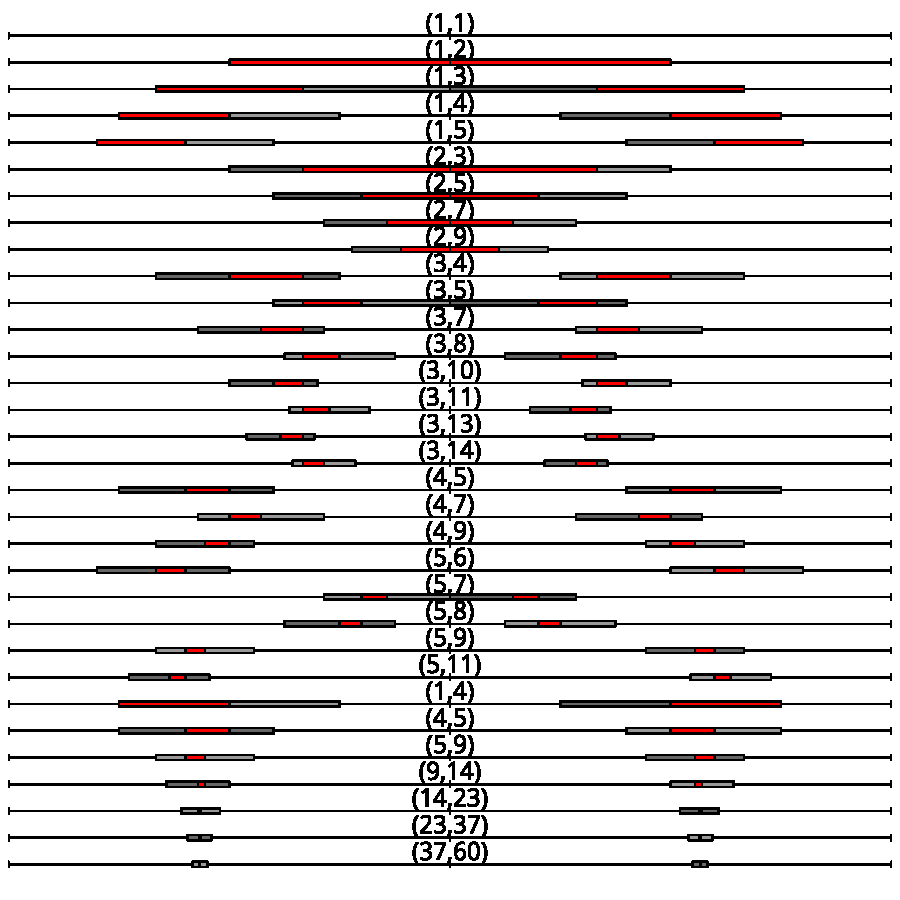
\includegraphics{figdir/fig-gi}
\caption{Generating intervals for a range of parastichy pairs.  Pink: subinterval on which pair is opposed; Light grey: subinterval on which pair is unopposed and $\Delta=+1$;Dark grey: unopposed and $\Delta=-1$. $d=\jhalf$ is not in any generating interval except for $(m,n)=(1,1)$; otherwise $\Delta$ in the opposed subinterval is the same as in the unopposed subintervals}
\label{fig:ogi}
\end{figure}
\end{center}




\clearpage
\section{van Iterson diagrams}





\begin{center}
\begin{figure}[H]
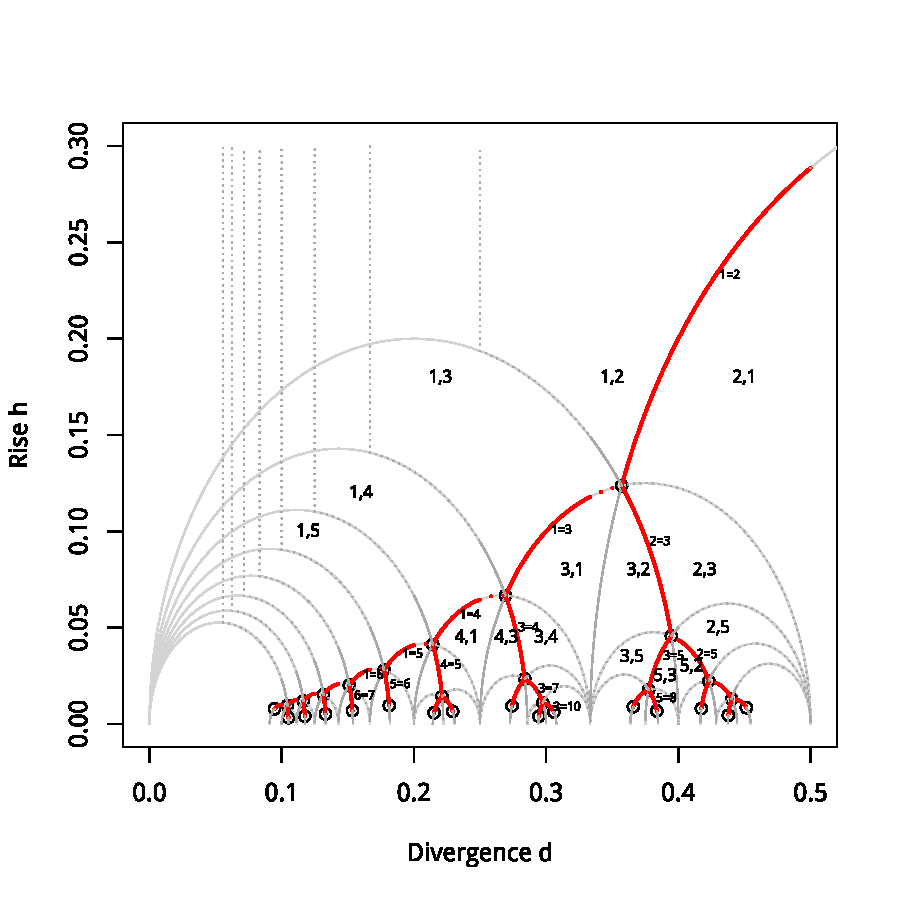
\includegraphics{figdir/fig-jsvanIterson}
\caption{Lattice space characterised by principal parastichy vectors as separated by the van Iterson tree}
\end{figure}
\end{center}


\section{Jean Theorem 4.2}



Jean uses a diagram like Figure~\ref{fig:ftp} to prove the FTP.


\begin{center}
\begin{figure}[H]
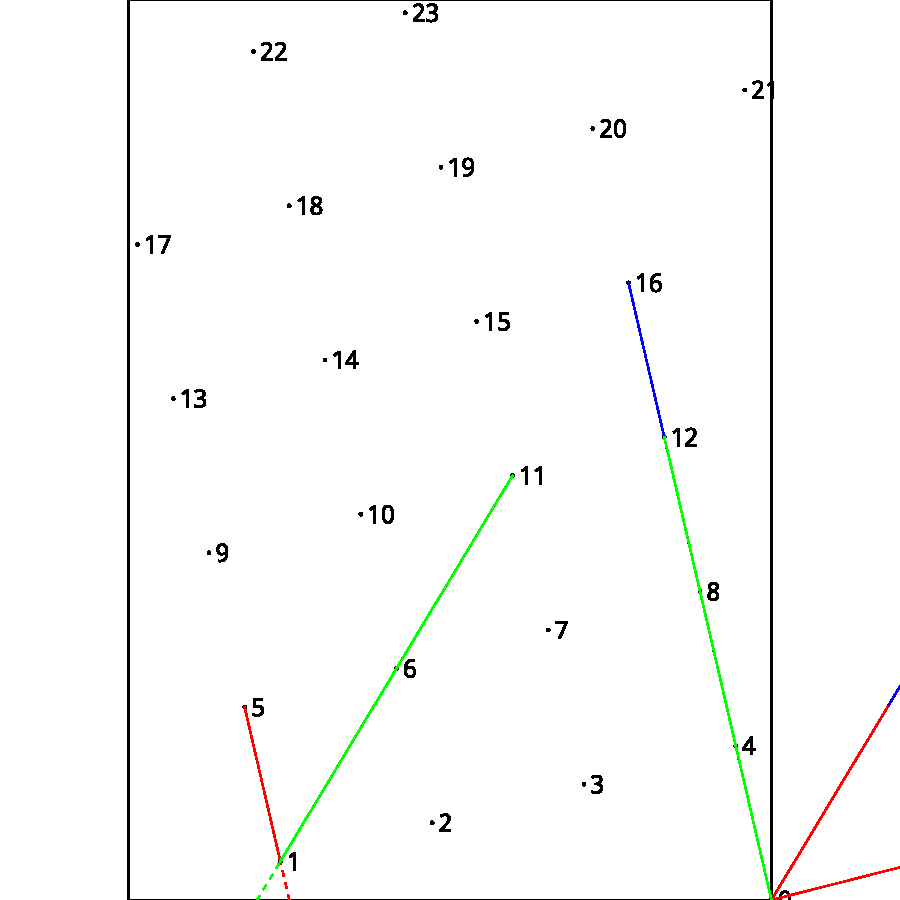
\includegraphics{figdir/fig-ftpfig}
\caption{Proof of the FTP}
\label{fig:ftp}
\end{figure}
\end{center}



\section{The lattice matrix}

Now we turn to an alternative description of the lattice. It can equally well be described by the coordinates of any
pair of vectors that generate it (Turing p64).

If those vectors are $(x,z)=(a,b)$ and $(c,d)$ respectively then the lattice matrix
is
\[
	\left( \begin{array}{ll}
	a & b \\ c & d
\end{array} \right )
=
\frac{1}{s}\left( \begin{array}{ll}
	sa & m \\ sc & n
\end{array} \right )
=
\frac{s_n}{s_d}\left( \begin{array}{ll}
	a' & m \\ b' & n
\end{array} \right )
\]
where $m=sb$ and $n=sd$ must be integers as the vertical components are multiple integers of the rise.
If $m$ and $n$ have a common factor, we can extract that into the rise via the scaling factor $s$, so we
can assume that they are coprime, and they are the parastichy pair for the matrix.

We try to keep the matrix entries integers, even under inversion, by recording the numerator and denominator of the scaling factor separately. To do this completely we should really keep an extra scaling factor for the $x$ component alone.


Note that we don't insist that the parastichy numbers are positive, but it would be a package bug if they were not integers.

We can also calculate what the width of the cylinder must be. The current code assumes the jugacy $J\equiv 1$.
\begin{Schunk}
\begin{Sinput}
> matrix.test <- matrix(c(2,1,-1,2),ncol=2,byrow=TRUE)
> PM.test <- as(matrix.test,"PhyllotaxisMatrix")
> 
> 
\end{Sinput}
\end{Schunk}



\begin{Schunk}
\begin{Sinput}
> GeometricalPhyllotaxis:::summary.PhyllotaxisMatrix.matrix(PM.test)
\end{Sinput}
\begin{Soutput}
|a	b|  = 1  /1   *  |  2	  1|
|c	d|               | -1	  2|
\end{Soutput}
\end{Schunk}


\subsection{Converting a genetic lattice to a matrix lattice}
It is easy to construct a matrix lattice from a genetic lattice by taking the first two points.

\subsection{Computing parameters from a matrix lattice}
Now we have all the parameters to construct a genetic spiral.
We can pull the rise out:

Since $m$ and $n$ are coprime there is a congruence: integers $k,l$ such that $km -l n=1$.

From the congruence we can find a point that has a rise of exactly 1, and so find the first point in
the genetic spiral.




That allows us to say more about the genetic form of the matrix
\begin{Schunk}
\begin{Sinput}
> GeometricalPhyllotaxis:::summary.PhyllotaxisMatrix.genetic(PM.test)
\end{Sinput}
\begin{Soutput}
(m,n)=(1,2); (3*1)-(1*2) = 1
getRise default generic called with object of class PhyllotaxisMatrix
Minimal cylinder radius 0.795775 circumference 5 
Divergence 2.51327 (144 degrees; Jean d 0.4)
Visible opposed divergence interval (6.28319,9.42478)
\end{Soutput}
\end{Schunk}


\subsection{Converting a lattice matrix to a genetic one}
Now it is simple to convert a lattice matrix to a genetic one.



So now we have two equvalent formulations of a lattice, one which privileges the genetic spiral and one which privileges a pair of
points in the lattice.



%\section{Plotting non-cylindrical lattices}

%<<fig>>=
%GeometricalPhyllotaxis:::.setup.grid(L=4)
%plot.from.LatticeMatrix(PM.test,y=4)
%@


Note that a lattice generated by $(\uvec,\vvec)$ is the same as one generated by $(\uvec+k\vvec,\vvec+l\uvec)$
so that two lattice matrices related by
\[
M_1 = \left( \begin{array}{ll} 1 & k \\ l & 1 \end{array}\right) M_2
\]
are equivalent.

\section{The principal parastichy vectors}



(Following Turing p56) The two vectors $\uvec$ and $\vvec$ from which
 we chose to generate the lattice are not necessarily the
shortest possible vectors in the lattice. By definition the first principal vector is the shortest nonzero vector in the lattice,
 and the second principal vector the shortest which is not a multiple of the first.

Observe that the first and second principal vectors must generate the lattice.
The parallelogram formed by the two principal vectors can be used to tile the plane, and
if there was a lattice point which is not generated by the first two principal vectors, it would
lie inside one of these parallelograms. But `a point within a parallelogram is always closer to one of
its vertices than are any of the vertices from one another' which would allow a vector of the lattice
shorter than the principal vectors in contradiction to their definition.


The area of the parallelogram formed by any two vectors $(\uvec,\vvec)$ in the lattice is $\Delta(\uvec,\vvec)$
\begin{eqnarray}
\Delta^2(\uvec,\vvec) &=& \uvec^2 \vvec^2 - (\uvec. \vvec)^2
\\
&=& \Delta^2(\uvec+k\vvec,\vvec+l\uvec)
\end{eqnarray}
and for vectors which generate the lattice it can be interpreted as the area per point
and so must be the same for any choice of generating vectors. This suggests a
systematic way to identify the principal vectors in a lattice. Since they minimise $\uvec^2\vvec^2$,
they must also minimise $ (\uvec. \vvec)^2 = \uvec^2 \vvec^2 - \Delta^2$. (Hence the latter part of Turing's theorem p57).
So we systematically
change $\uvec$ and $\vvec$ always trying to minimize $\left|\uvec. \vvec\right|$.
One easy way to do that is to look at the sum or difference of $\uvec$ and $\vvec$, and
by insisting that $\uvec. \vvec>0$ the shorter of those is $\uvec-\vvec$ (Observe
that $0<\uvec.\vvec < \uvec^2/2 \iff  \left|\vvec\right|<\left|\uvec-\vvec\right|<\left|\uvec+\vvec\right|$.)


Specifically, start with  $\uvec$ and  $ \vvec$, and relabel and change the sign of
$\vvec$ if necessary so that  $\uvec^2\leq\vvec^2$ and $\uvec. \vvec>0$. That guarantees
$\left|\vvec\right|<\left|\uvec+\vvec\right|$ but it might be that
$\uvec.\vvec>\uvec^2/2 \iff \left|\vvec\right|>\left|\uvec-\vvec\right|$ in which case replace $(\uvec,\vvec)$ by
$(\uvec,\vvec-\uvec)$. That reduces $\uvec.\vvec$ by $\uvec^2$, so
 $\left|\uvec.\vvec\right|$ will
be reduced.  Now may need to relabel and change signs again, which will not change this modulus.


Eventually, will have a $\uvec$ and  $ \vvec$ such that
$0<2\uvec.\vvec < \uvec^2 <\vvec^2$. But Turing p57 shows such a pair are the first two parastichy vectors.

For integers $m,n\geq 1$
\begin{eqnarray}
(m\uvec+n\vvec)^2 - (\uvec-\vvec)^2
 &=& m^2 \uvec^2 +n^2 \vvec^2 + 2 mn \uvec.\vvec - (\uvec^2+\vvec^2-2\uvec.\vvec)
\\
&=& (m^2 -1)\uvec^2 +(n^2-1) \vvec^2 + 2( mn+1) \uvec.\vvec
\\
&\geq& (m^2-\left|mn\right|+1)\uvec^2 + (n^2-1)\vvec^2
\\
&\geq& (m^2-\left|mn\right|+n^2)\uvec^2
\\
&=& ((\left|m\right|-\left|n\right|)^2+\left|mn\right| )\uvec^2
\\
&\geq&0
\end{eqnarray}
Since $0< \uvec^2 <\vvec^2<(\uvec-\vvec)^2$ there are no other vectors of the lattice shorter
than any of these three which are not multiples of $\uvec$ or $\vvec$, so they are the
the first three parastichy vectors.

In matrix terms, if the initial lattice matrix has $\uvec^2>\vvec^2$ then multiply it by
\[
\left( \begin{array}{ll}0 & 1 \\ 1 & 0 \end{array}\right)
\]
then if $\uvec.\vvec<0$ multiply it by
\[
\left( \begin{array}{ll} 1 & 0  \\ 0 & -1 \end{array}\right)
\]
and then if $\uvec.\vvec>\uvec^2/2$ multiply it by
\[
\left( \begin{array}{ll} 1 & 0  \\ -1 & 1\end{array}  \right)
\]
which is guaranteed to reduce the modulus of $\uvec.\vvec$.

So now we can find the Principal vectors in a matrix lattice and convert to a representation
in those vectors. We adopt the convention that the first principal vector has a positive $z$ component and thus the first parastichy number is positive.


This allows us to say more about matrix objects:
\begin{Schunk}
\begin{Sinput}
> print(PM.test)
\end{Sinput}
\begin{Soutput}
An object of class "PhyllotaxisMatrix"
Slot "nScale":
[1] 1

Slot "dScale":
[1] 1

Slot "Coord":
     [,1] [,2]
[1,]    2    1
[2,]   -1    2

Slot "Rho":
[1] 0.7957747

Slot "origin":
[1] 0 0

Slot "L":
[1] 50
\end{Soutput}
\begin{Sinput}
> 
\end{Sinput}
\end{Schunk}
\subsection{Example of converting a lattice matrix to its principal form}
\begin{Schunk}
\begin{Sinput}
> set.seed(1)
> Prand <- as(matrix(sample(100,4),ncol=2,byrow=TRUE),"PhyllotaxisMatrix")
> print(Prand)
\end{Sinput}
\begin{Soutput}
An object of class "PhyllotaxisMatrix"
Slot "nScale":
[1] 1

Slot "dScale":
[1] 1

Slot "Coord":
     [,1] [,2]
[1,]   27   37
[2,]   57   89

Slot "Rho":
[1] 46.79155

Slot "origin":
[1] 0 0

Slot "L":
[1] 50
\end{Soutput}
\begin{Sinput}
> print(GeometricalPhyllotaxis:::makePrincipalPhyllotaxisMatrix (Prand))
\end{Sinput}
\begin{Soutput}
An object of class "PhyllotaxisMatrix"
Slot "nScale":
[1] 1

Slot "dScale":
[1] 1

Slot "Coord":
     [,1] [,2]
[1,]    3   15
[2,]  -18    8

Slot "Rho":
[1] 46.79155

Slot "origin":
[1] 0 0

Slot "L":
[1] 50
\end{Soutput}
\begin{Sinput}
> 
\end{Sinput}
\end{Schunk}

\subsection{Plotting the principal vectors in a lattice}
Now we can generate principal vectors for  a lattice we can include those in the plots.

\subsection{Do the principal vectors always oppose?}
No:

\begin{Schunk}
\begin{Sinput}
> Podd <-  as(matrix(c(7,1,2,8),ncol=2,byrow=TRUE),"PhyllotaxisMatrix")
> print(Podd)
\end{Sinput}
\begin{Soutput}
An object of class "PhyllotaxisMatrix"
Slot "nScale":
[1] 1

Slot "dScale":
[1] 1

Slot "Coord":
     [,1] [,2]
[1,]    7    1
[2,]    2    8

Slot "Rho":
[1] 8.594367

Slot "origin":
[1] 0 0

Slot "L":
[1] 50
\end{Soutput}
\end{Schunk}
\begin{Schunk}
\begin{Sinput}
> Podd@L <- 70
> Podd@lhsOrigin <- FALSE
> plotPhyllotaxis(Podd)
\end{Sinput}
\end{Schunk}

\begin{Schunk}
\begin{Sinput}
> Pnotcoprime <- as(matrix(c(-1,2,2,4),ncol=2,byrow=TRUE),"PhyllotaxisMatrix")
> print(Pnotcoprime)
\end{Sinput}
\begin{Soutput}
An object of class "PhyllotaxisMatrix"
Slot "nScale":
[1] 2

Slot "dScale":
[1] 1

Slot "Coord":
     [,1] [,2]
[1,] -0.5    1
[2,]  1.0    2

Slot "Rho":
[1] 1.27324

Slot "origin":
[1] 0 0

Slot "L":
[1] 50
\end{Soutput}
\end{Schunk}




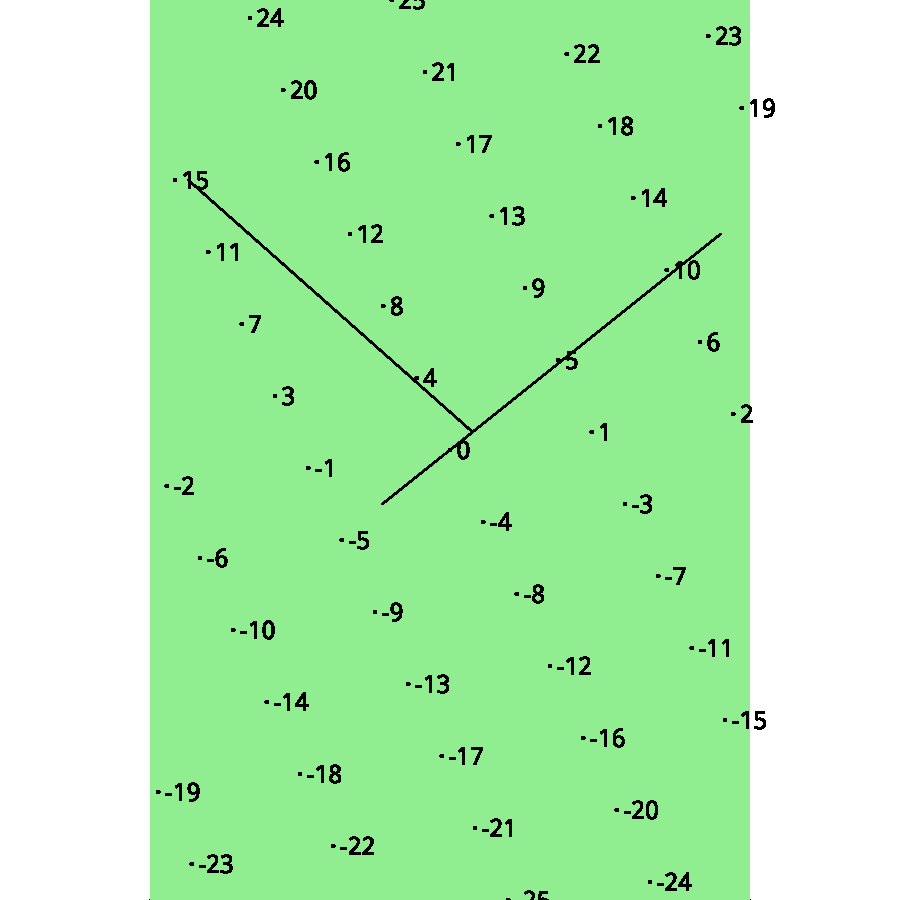
\includegraphics{figdir/fig-038}

\section{Jean computation}



\begin{Schunk}
\begin{Sinput}
> tau <- (1+sqrt(5))/2
> divergence <- 1/tau^2
> JeanComputation(1/tau^2)
\end{Sinput}
\begin{Soutput}
   0 |   1 
   1 |   2 

   0   1 |   1 
   1   3 |   2 

   0   1 |   2   1 
   1   3 |   5   2 

   0   1 |   2   3   1 
   1   3 |   5   7   2 

   0   1   3 |   2   3   1 
   1   3   8 |   5   7   2 

   0   1   4   3 |   2   3   1 
   1   3  11   8 |   5   7   2 

   0   1   4   3 |   2   5   3   1 
   1   3  11   8 |   5  12   7   2 

   0   1   4   3 |   5   2   5   3   1 
   1   3  11   8 |  13   5  12   7   2 

   0   1   5   4   3 |   5   2   5   3   1 
   1   3  14  11   8 |  13   5  12   7   2 

   0   1   6   5   4   3 |   5   2   5   3   1 
   1   3  17  14  11   8 |  13   5  12   7   2 

   0   1   6   5   4   3 |   5   7   2   5   3   1 
   1   3  17  14  11   8 |  13  18   5  12   7   2 

   0   1   6   5   4   7   3 |   5   7   2   5   3   1 
   1   3  17  14  11  19   8 |  13  18   5  12   7   2 

   0   1   6   5   4   7   3   8 |   5   7   2   5   3   1 
   1   3  17  14  11  19   8  21 |  13  18   5  12   7   2 
     [,1] [,2]
[1,]    1    2
[2,]    3    2
[3,]    3    5
[4,]    8    5
[5,]    8   13
[6,]   21   13
\end{Soutput}
\begin{Sinput}
> 
> 
> 
\end{Sinput}
\end{Schunk}




\begin{Schunk}
\begin{Sinput}
> PG.Fibonacci <-  newPhyllotaxisGenetic(Rise=1,Divergence=(2*pi)/tau^2,Rho=40/(2*pi),Jugacy=1)
> plotPhyllotaxis(PG.Fibonacci,y=50,bottomOrigin=TRUE,doNumbers=TRUE)
> grid.lines(x=c(0,0),y=c(0,50),default.units="native")
\end{Sinput}
\end{Schunk}
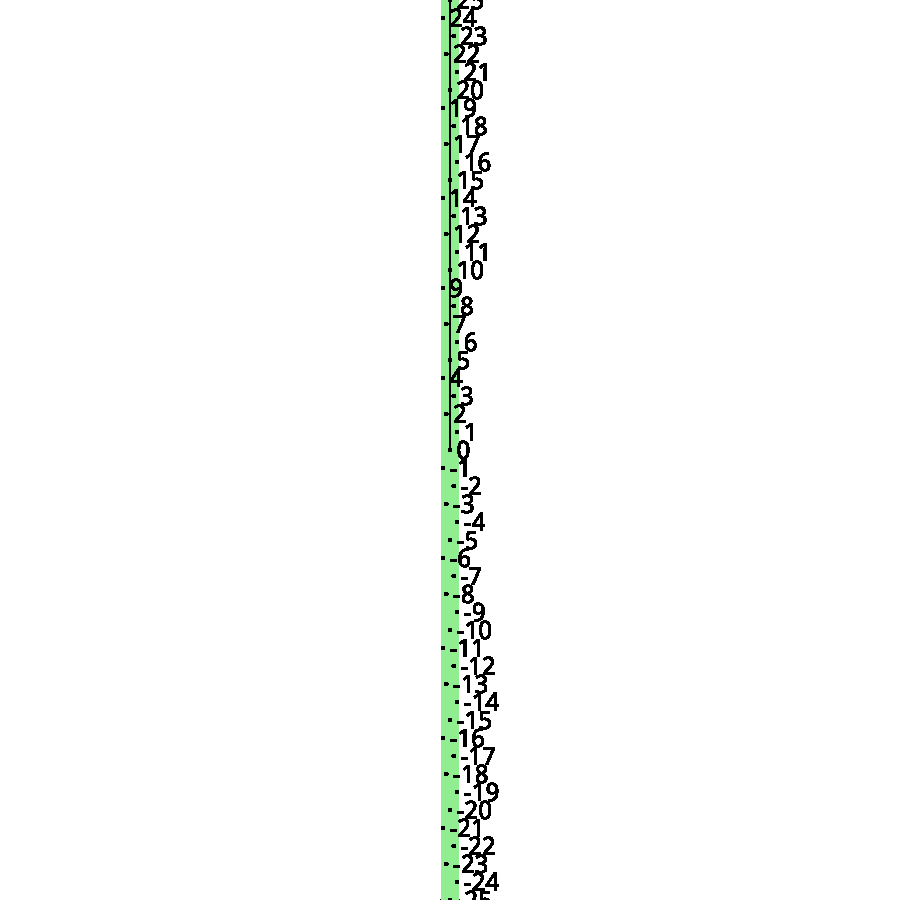
\includegraphics{figdir/fig-fibfig}



\section{Touching circles}
We can take the length of the first parastichy vector as the diameter
of the largest  circles which can be packed on the cylinder with centres given by the lattice:
what Turing and van Iterson called `touching circle phyllotaxis'.
An arbitrary lattice is not in general a close packing for a touching circle phyllotaxis compared to other packings of circles
with the same radius:

\begin{Schunk}
\begin{Sinput}
> plotPhyllotaxis(PG.test,y=10,doCircles=TRUE)
\end{Sinput}
\end{Schunk}
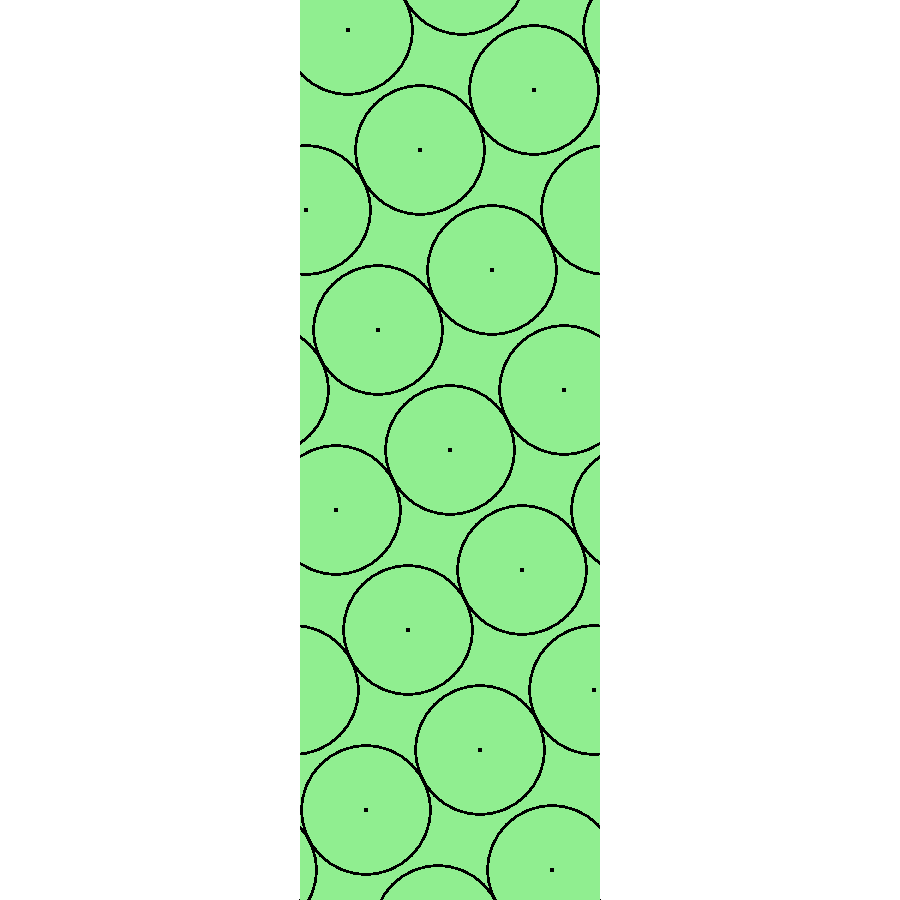
\includegraphics{figdir/fig-041}


\section{Facets}
Similarly we can construct the parallelogram formed by the principal vectors and facet the cylinder with it.
\begin{Schunk}
\begin{Sinput}
> plotPhyllotaxis(PG.test,y=10,doFacets=TRUE)
\end{Sinput}
\end{Schunk}
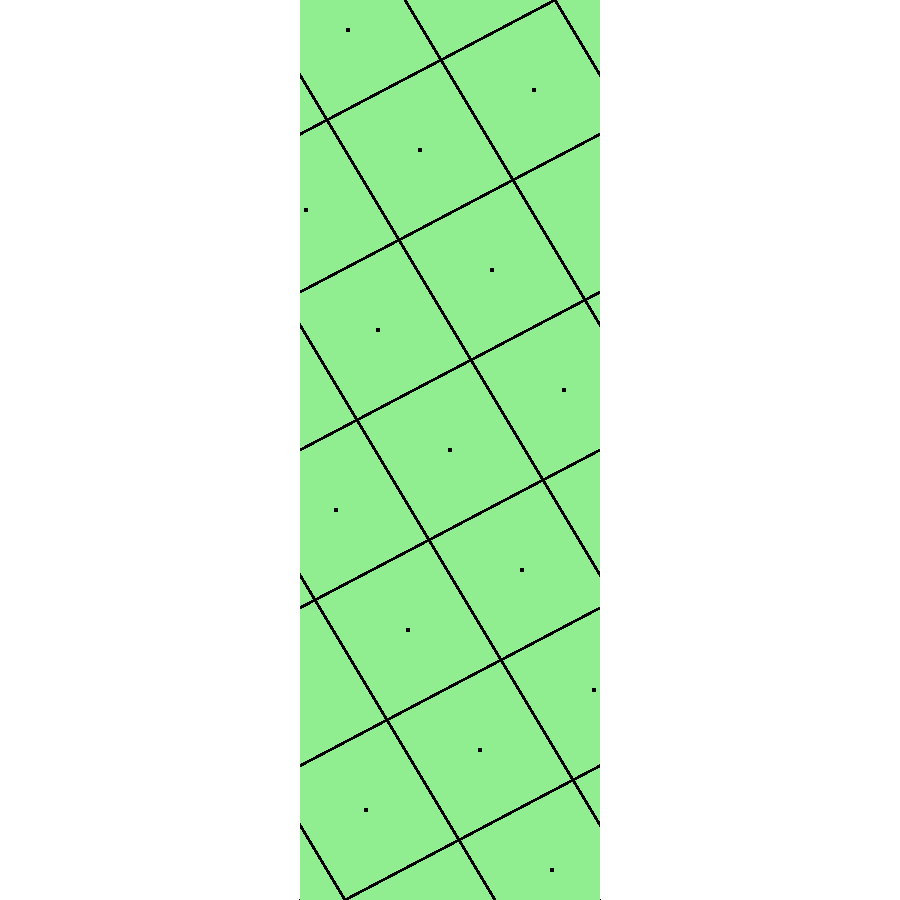
\includegraphics{figdir/fig-042}



\section{Notation}



\begin{tabular}{lccc}
& Turing\cite[p54]{turing:1952} &  Jean\cite{jean:1994} & \cite{abop:1991} \\
\hline
Divergence angle & $0 \leq \alpha \leq 2\pi $\\

Scaled divergence & $0 \leq d_T=\alpha/2\pi \leq 1$ & $0 \leq d=\alpha/2\pi \leq 1$ & \\
Jugacy & $J=\kappa/2\pi$ & Fixed at 1 & \\
Rise & $\eta$ & $v$ & \\
Cylinder circumference &$2\pi\rho$& $u=2\pi\rho$ & \\
Normalised cylinder && $r=2\pi\rho/\eta$\\
\end{tabular}
\bibliography{GPpackage}
\end{document}

